\documentclass[a4paper]{report}

\usepackage[utf8]{inputenc} %Accent
%\usepackage{libertine} %Font
\usepackage[english, francais]{babel} %langue

\usepackage{graphicx} %Include fig
\usepackage{caption} %center the caption
\usepackage{subfig} %Include subfig
\usepackage{lastpage} %ref LastPage 
\usepackage{fancyhdr} % headers,footers
\usepackage{multicol} % minipages
\usepackage{textcomp} 
\usepackage{lscape}   %Format paysage
\usepackage{fancybox} %Image arrière plan
\usepackage{amsmath} %\mathbb, \mathit...
\usepackage{amssymb} 
\usepackage{color} %couleurs
\usepackage{float}
\usepackage[hidelinks]{hyperref} %Liens intradoc et url
\usepackage{titlepic}

%\usepackage{algorithm}
%\usepackage{algorithmic} %Algo en pseudo code
%\usepackage{algorithm2e} %for psuedo code

%\usepackage{boxedminipage} %Surligner

%\newcounter{apppage} % Annexes

%Dossier contenant les figures
\graphicspath{{../fig/}}

%Mise en page
\voffset -1.5 cm
\textheight 24.3 cm
\topmargin 0 cm
\headheight 0 cm
%\headsep 0.6 cm
\textwidth 16.5 cm
\evensidemargin 0 cm
\marginparsep 0 cm
\marginparwidth 0 cm
\oddsidemargin -.5 cm

%Titre
\title{Speech Signal Processing\\Report\\Project n°2}
\author{Félix Côte \and Antoine Honoré}



%Type de numérotation des sections & sous-sections
\renewcommand{\thesection}{\Roman{section}}
\renewcommand{\thesubsection}{\thesection.\arabic{subsection}}

%\renewcommand\thesubfigure{(\alph{subfigure})}
\setlength{\parindent}{0cm}
\setlength{\parskip}{1ex plus 0.5ex minus 0.2ex}
\newcommand{\hsp}{\hspace{20pt}}
\newcommand{\HRule}{\rule{\linewidth}{0.5mm}}

%email
\newcommand{\email}[1]{\href{mailto:#1}{\color{blue} \textsf{#1}}}

%Bibliography
\bibliographystyle{apalike}

%Environnement insersion image
\newcommand{\img}[3]{\begin{figure}[!h] \centering \includegraphics[scale=#2]{#1}\captionsetup{justification=centering} \caption{#3} \label{#1} \end{figure}}
  % commande \img{nom image}{scale}{legende}

%TODO
\newcommand{\todo}[1]{{ \Large \textbf{ \colorbox{yellow}{\color{blue} TODO:}}~#1}}

%pushright
\newenvironment{pushright}[1]{\textbf{#1}
\begin{itemize}\item[\hspace{12pt}]}{\end{itemize}
}

%%%%%%%%%%%%%%%%%%%%%%%%%%%%%%%%%%%%%%%%%%%%%%%%%%%%%%%%%%%%%%
%%%%%%%%%%%%%%%%%%%%%%%%%%%%%%%%%%%%%%%%%%%%%%%%%%%%%%%%%%%%%%
%%%%%%%%%%%%%%%%%%%%%%%%%%%%%%%%%%%%%%%%%%%%%%%%%%%%%%%%%%%%%%
\pagestyle{fancy}  % Activation en-tête et pied de page

%En-tête
\fancyhead[L]{Félix Côte \& Antoine Honoré - Speech Signal Processing  Project n°2}
%\fancyhead[C]{}
%\fancyhead[R]{}
% Pied de page
\newcommand{\width}{3cm}
%\fancyfoot[L]{ \includegraphics[width=\width]{logo-gipsa} }
\fancyfoot[C]{ \thepage~/~\pageref{LastPage} }
%\fancyfoot[R]{ \includegraphics[width=\width]{logo-phelma} }

%\titlepic{\includegraphics[scale=0.6]{kth-logo}}

\begin{document}

%%%%%%%%%%%%%%%% TITLE %%%%%%%%%%%%%%%%
\begin{titlepage}
  \begin{sffamily}
    \begin{center}

      \textsc{ }\\[1.5cm]

      % % Title
      % \vspace{3cm}
      \HRule \\[0.4cm]
      { \Huge \bfseries Speech Signal Processing\\ Project n°2\\[0.4cm] }
      \HRule \\[2.5cm]
      \textsc{\LARGE Report}~\\[2.5cm]
% Authors
      \begin{minipage}{0.4\textwidth}
        \begin{flushleft} \large
          \emph{\textbf{Student}}\\
          Antoine \textsc{Honoré}\\
          \email{honore@kth.se}
          ~\\~\\~\\
        \end{flushleft}
      \end{minipage}
      \hfill
      \begin{minipage}{0.4\textwidth}
        \begin{flushright} \large
          \emph{\textbf{Student}}\\
          Félix \textsc{Côte}\\
          \email{@kth.se}
        \end{flushright}
      \end{minipage}
      % \includegraphics[scale=0.5]{kth-logo}

     

      \vfill

      % Bottom of the page
      {\large 2015/2016 Period 3}

    \end{center}
  \end{sffamily}

\end{titlepage}


%%% Local Variables:
%%% TeX-master: "master"
%%% End:
%%%%%%%%%%%%%%%%%%%%%%%%%%%%%%%%%%%%%%%%%%%%%%%%%%%%%%%%%%%%%%%%
%%%%%%%%%%%%%%%%%%%%%%%%%%%%%%%%%%%%%%%%%%%%%%%%%%%%%%%%%%%%%%%%
%%%%%%%%%%%%%%%%%%%%%%%%%%%%%%%%%%%%%%%%%%%%%%%%%%%%%%%%%%%%%%%%
%%%%%%%%%%%%%%%%%%%%%%%%%%%%%%%%%%%%%%%%%%%%%%%%%%%%%%%%%%%%%%%%
%%%%%%%%%%%%%%%%%%%%%%%%%%%%%%%%%%%%%%%%%%%%%%%%%%%%%%%%%%%%%%%%
\section{Introduction}

\section{Uniform Scalar Quantizer}
In this part we implement the most basic quantizer. The USQ is entirely defined with three parameters:\begin{itemize}
\item $n_{bits}$, the number of bits used to code one sample. $2^{n_{bits}}$ is the number of output value;
\item m, the mean of the output values;
\item xmax the maximum of the output values;
\end{itemize}

In this part we tried m=0 and m=1.5. The result that we got plotting the input sigal versus the input signal is presented on figure \ref{USQ_INOUT}.

\begin{figure}[!h]
  \centering
\subfloat[m = 0]{  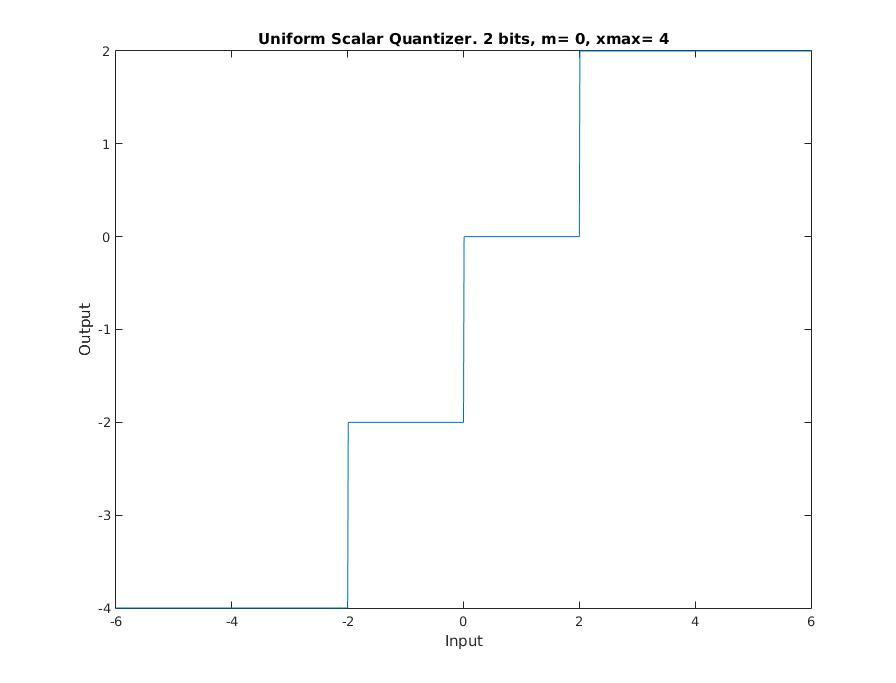
\includegraphics[scale=.3]{USQ_INOUT_m0} }
\subfloat[m = 1.5]{  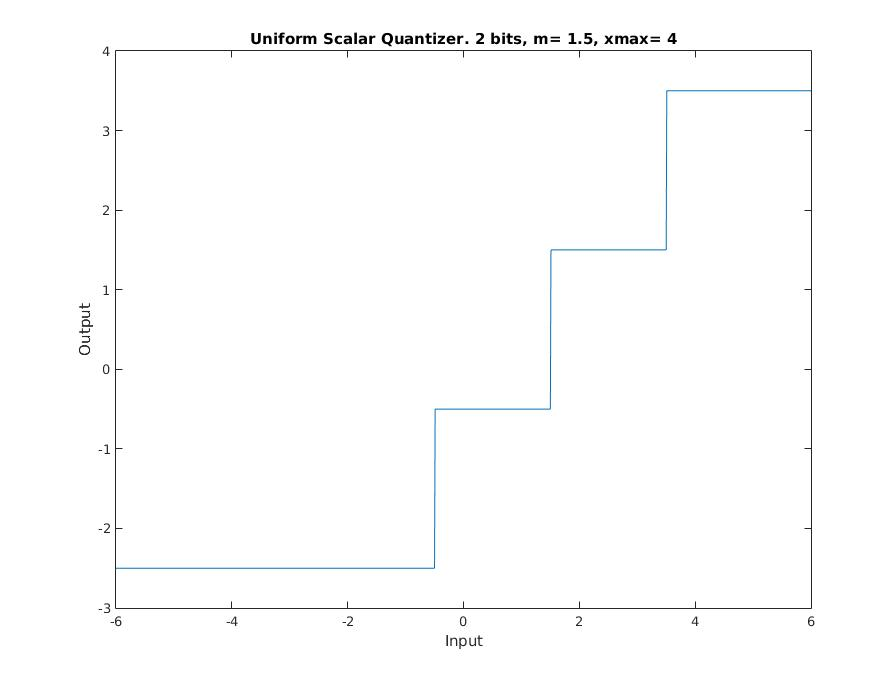
\includegraphics[scale=.3]{USQ_INOUT_m15} }

  \caption{Input vs Output}
  \label{USQ_INOUT}
\end{figure}
To compare the two settings, we need to plot the distorsion-rate curve and compare the performance. This is presented on figure \ref{USQ_RateDistCurve}.

\begin{figure}[!h]
  \centering
  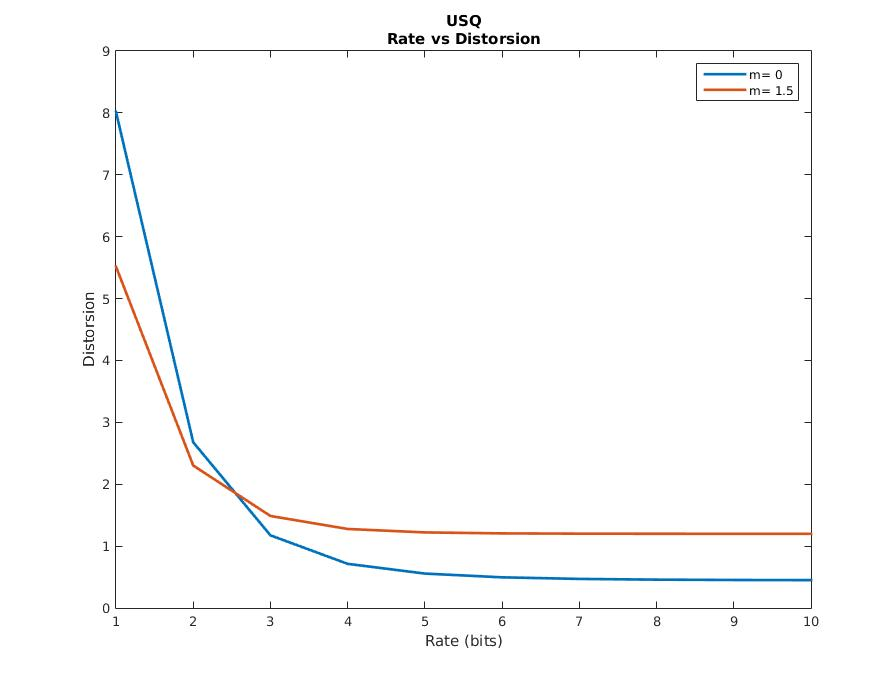
\includegraphics[scale=.35]{USQ_RateDistCurve}
  \caption{Rate-Distorsion curve for two values of m.}
  \label{USQ_RateDistCurve}
\end{figure}


\pagebreak
\section{Parametric coding of speech}
dsd
\end{document}
